\subsection{ZDC}

The aim of the ZDC upgrade is to cope with the high collision rate foreseen after LHC LS2 upgrade. The calorimeters sustained well irradiation during RUN1/2 operation, therefore don't need to be replaced. The two items that required attention were the consolidation of the infrastructure and the upgrade of the readout system.

The first item required two main actions. Firstly it involved the upgrade of the control electronics of the movable platform that bring the ZDC calorimeters in a garage position where it is shielded by potential beam losses during beam injection or adjustment operations and allow to align them with the neutron (proton) spot during data taking. A second action involved the installation of additional power supplies for the voltage dividers of the ZDC photomutipliers to stabilize the gain in the high event rate conditions that are foreseen. 

The main upgrade activity concerned a new readout system based on faster electronics. In fact the RUN1/2 readout electronics was based on VME QDCs with a conversion time of $\sim\SI{10}{\micro\second}$ that cannot cope with a $\SIrange[range-units=single,range-phrase=\div]{50}{100}{\kilo\hertz}$ event rate without dead time (taking also into account a possible luminosity increase beyond the LS3 baseline). Moreover, in order to fully exploit the ALICE physics potential in ultra-peripheral heavy ion collision, the ZDC aims at taking data in continuous (autotrigger) readout mode. This operating condition is particularly challenging since the ZDC has acceptance not only to nucleon emission from hadronic interactions but also to the ones resulting from electromagnetic dissociation \cite{Pshenichnov2001,Pshenichnov2011,ALICE:2012aa} that has $\sim 50$ times higher cross section for Pb-Pb collisions at LHC energies. The designed Pb-Pb readout rate of $\SI{100}{\kilo\hertz}$ will be accompained by an additional $\sim\SI{5}{\mega\hertz}$ event rate, mostly uncorrelated among the two ZN, resulting from electromagnetic interactions that do not involve barrel detectors.

Thanks to the low number of channels to be instrumented, the new readout system is based on commercial digitizers, in particular ALICE will use FMC digitizers that allow a continuous sampling of the signal waveform followed by a real time analysis on a FPGA. 
Thanks to the adequate bandwidth available through the FMC connection from the digitizer to the FPGA the full waveform can be analyzed. Fast trigger and selection algorithms are executed on the FPGA and the interesting portions of waveform are transferred to the acquisition and reconstruction system through optical GBT links.

To preserve the time and charge resolution 
%of the present system
and to match the bandwidth of the ZDC signals, the digitizers should have about $\SI{12}{\bit}$ resolution (with an ENOB of $\sim\SI{10}{\bit}$) with a sampling frequency of
% $\SIrange[range-units=single,range-phrase=\div]{0.5}{1}{\giga\sps}$
$\SIrange[range-units=single,range-phrase=\div]{0.5}{1}{\giga\hertz}$. Since the PM signal is unipolar the digitizer has to be DC coupled (and this reduces the number of useful models available on the market). After evaluating a few modules it was chosen the ADC3112 FMC \cite{IOXOSADC3112} mounting digitizer ADS5409 \cite{TIADS5409}. The FMC is hosted on the carrier IFC\_1211 \cite{IOXOSIFC1211} with a Kintex UltraScale XCKU40 FPGA. The ADC3112 on-board oscillator is locked to the LHC revolution frequency recovered from GBT link and dispatched through the FMC connector. The ADC will acquire 24 samples per bunch crossing, therefore it will run at a frequency of
% $\sim\SI{960}{\mega\sps}$
$\sim\SI{960}{\mega\hertz}$. In order to reduce the data size the low pass filtering with digital downsampling is enabled on the ADC. This has the benefit of improving the measurement accuracy by averaging over the even and odd samples without the need to correct for the slightly different gain and offset that is present on this type of ADC. The data throughput to the FPGA will therefore be reduced to 12 samples per bunch crossing at $\sim\SI{480}{\mega\sps}$, simplifying the firmware design.

A critical aspect of the ZDC operation in RUN3 is triggering at high rate in \PbPb with bunch spacing reduced to $\si{50}$ or $\SI{25}{\nano\second}$ since the PM signal will be comparable or longer than the bunch spacing. This is complicated by the large signal dynamics (from a one to $\sim60$ neutrons in the acceptance of the neutron calorimeters). In order to identify the presence of a signal a differential trigger algorithm has been developed. Samples at different times are compared (sample $y_{\textrm{i}}$ with sample $y_{\textrm{i+shift}}$ where $\textrm{shift}$ is a tunable parameter from 3 to 5 samples). If three successive differences are above threshold $th$, i.e. $\left(y_{\textrm{i}}-y_{\textrm{i+shift}}\right)>th\,\&\,\left(y_{\textrm{i+1}}-y_{\textrm{i+shift+1}}\right)>th\,\&\,\left(y_{\textrm{i+2}}-y_{\textrm{i+shift+2}}\right)>th$ 
the trigger condition is satisfied, effectively rejecting fake triggers due to electronic noise, and the bunch is flagged for acquisition. This autotrigger condition drives the acquisition in continuous readout mode while in triggered mode the readout system acquires data regardless of the autotrigger flag. The same flags are used also to measure the interaction rate that is used to estimate the instantaneous luminosity.

The measurements of signal arrival time and amplitude need to take into account the baseline (pedestal) oscillations and the possible presence of a signal in an earlier bunch crossing (pile-up).

Two methods for pedestal evaluation have been implemented. Given the bunch structure of LHC that alternates ``trains'' of colliding bunches to ``gaps'' where no collisions can occur, it is possible to measure the pedestal considering portions of the digitized data where no collision can occur. These are identified by a filling map uploaded on the frontend at each fill. Using this information the pedestal average for each LHC orbit is computed and then transmitted on GBT. This allows taking into account a possible low frequency drift of the baseline and obtaining an accurate reference. A second method allows to effectively subtract pedestal in presence of noise at higher frequencies. For each trigger (or autotrigger), in addition to the bunch where the signal peaks ($BC_0$), the 12 samples of the preceding bunch crossing ($BC_{-1}$) will be transferred in order to evaluate and subtract the pedestal, allowing to correctly subtract pedestal in case of significant discrepancy with the orbit average computed with the first method.

For what concerns the pile-up from a signal in an earlier bunch crossing, in autotrigger mode all ZDC signals are transmitted and reconstructed, allowing to identify and correct for pile-up. On the other hand, in triggered mode, the firmware ensures that the information on the signal inducing pile-up is not lost due to trigger selectivity. Consequently for each triggered bunch crossing up to four bunch crossings will be transferred: the triggered and the preceding one (pedestal evaluation) and additionally $BC_{-2}$ and $BC_{-3}$ in case a pile-up signal is detected.

During \PbPb data taking in 2018 a prototype of the ZDC system was tested in parallel to the ALICE data acquisition by using a custom system based on a Xilinx evaluation board readout with Labview. An example of the achieved performances is shown in Fig. \ref{fig:zdc-signals}. The resolution on $\SI{2.76}{\tera\electronvolt}$ single neutron emission detected by ZNC is $\sim17\%$, with an improvement w.r.t. the $\sim20\%$ of previous electronics. The time resolution w.r.t. the ALICE L0 trigger is $\sim\SI{0.35}{\nano\second}$, a value that is comparable with the performance of the previous system.

\begin{figure}
    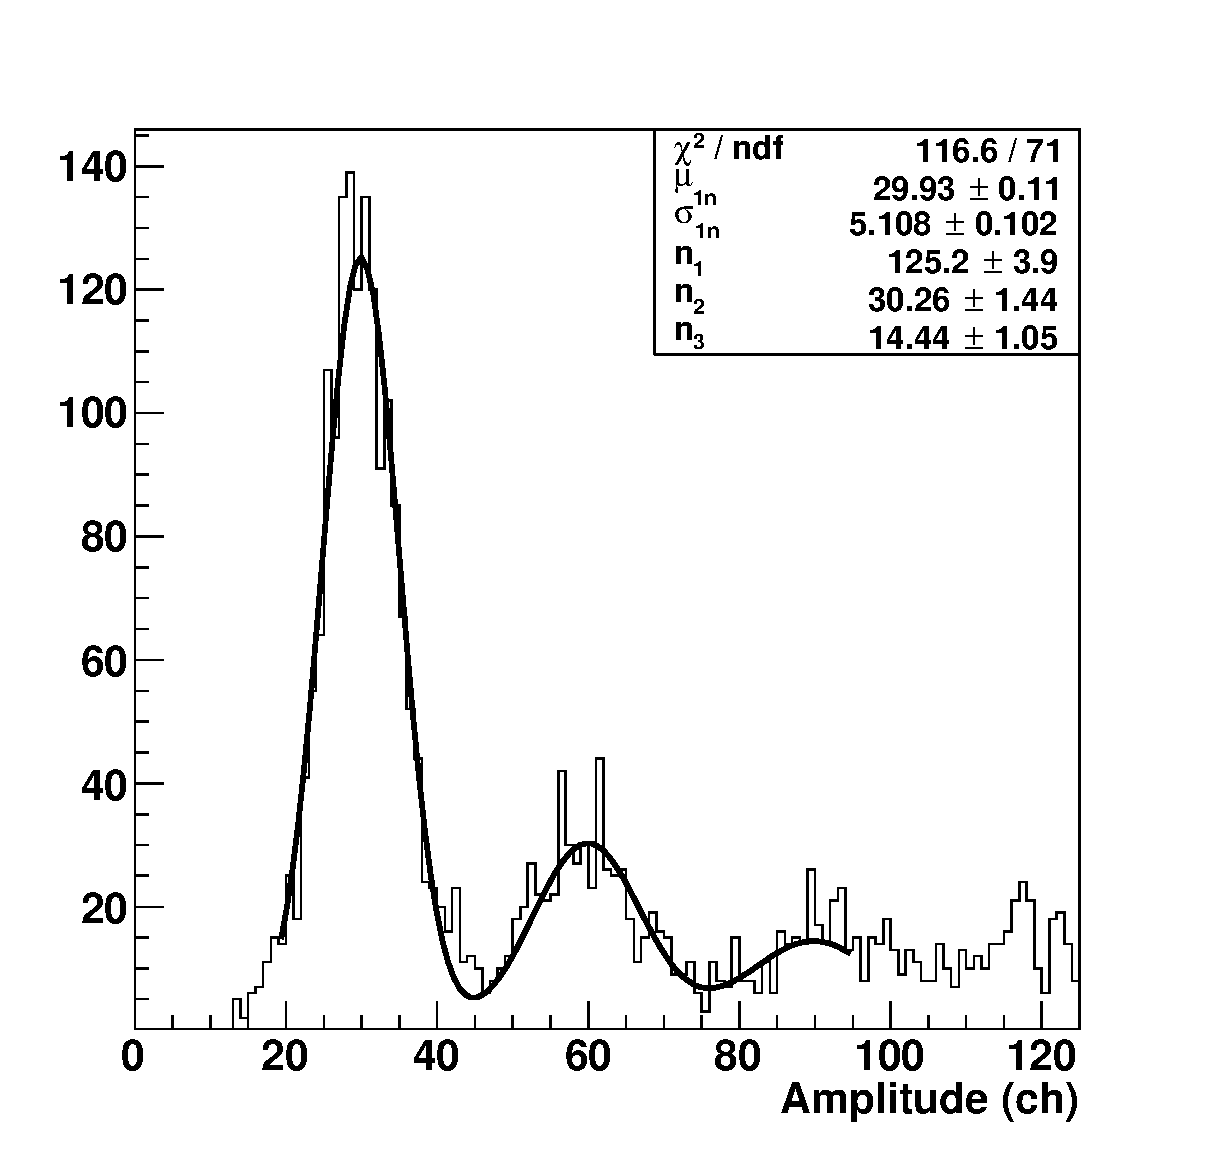
\includegraphics[viewport=0bp 0bp 569.4bp 736.111bp,clip,width=0.5\columnwidth]{zdc/fill_7457_dcmtnon_1n_resolution}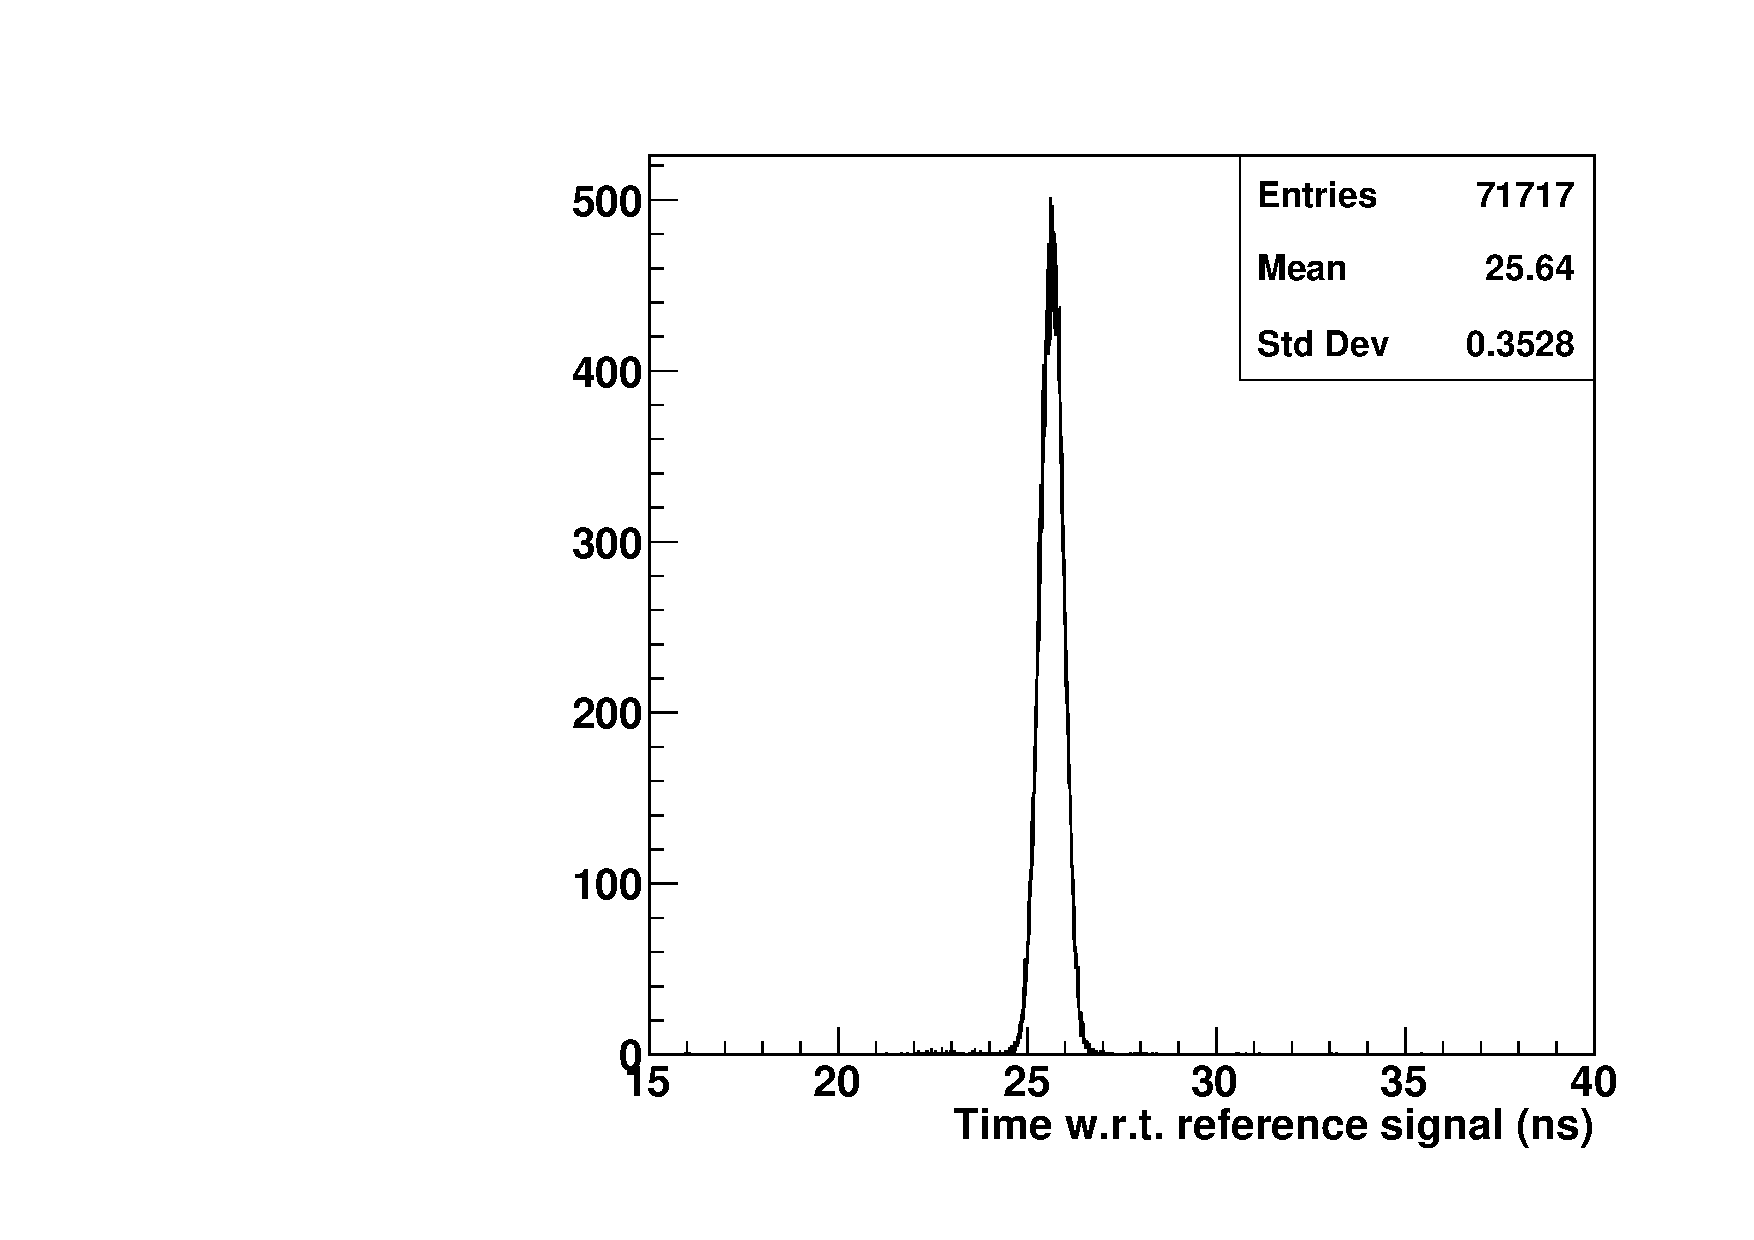
\includegraphics[viewport=0bp 0bp 569.4bp 736.111bp,clip,width=0.5\columnwidth]{zdc/run296549-part0-dcmtnon-d20181120-h1230_znctc_time}

    \caption{\label{fig:zdc-signals}Analysis of the performance of the digitizer during Pb-Pb 2018 data taking in the operating conditions chosen for RUN3. On the left plot: the lower part of the triggered spectrum of ZNC common photomultiplier in Pb-Pb collisions where the emission of a single $\SI{2.76}{\tera\electronvolt}$ neutron  and multiples are visible. The autotrigger algoritm effectively rejects pedestal events. On the right plot: the arrival time of ZNC common photomultiplier
    signals w.r.t. the reference ALICE L0 trigger signal.}
\end{figure}
    
    
